\documentclass[12pt,compress,aspectratio=169]{beamer}
\usetheme{metropolis}
\setbeamersize{text margin left=.8cm,text margin right=.8cm}
\usepackage[lf]{carlito}
\usepackage{amsmath,bm}
\usepackage{siunitx}
\usepackage{tikz}
\usepackage{mathpazo}
\usepackage{xcolor,colortbl}

\usetikzlibrary{patterns}

\setmonofont{Liberation Mono}
\setlength{\parskip}{0pt}
\setlength{\itemsep}{0pt}
\renewcommand{\baselinestretch}{1}

\sisetup{
  per-mode=symbol
}
\tikzset{>=latex}

\title{Topic 6: Rotational Motion of a Rigid Body}
\subtitle{Advanced Placement Physics 1}
\author[TML]{Dr.\ Timothy Leung}
\institute{Olympiads School}
\date{Last Updated: \today}

\newcommand{\pic}[2]{\includegraphics[width=#1\textwidth]{#2}}
\newcommand{\mb}[1]{\ensuremath\mathbf{#1}}
\newcommand{\iii}{\bm{\hat{\imath}}}
\newcommand{\jjj}{\bm{\hat{\jmath}}}
\newcommand{\kkk}{\bm{\hat{k}}}
\newcommand{\eq}[2]{\vspace{#1}{\Large\begin{displaymath}#2\end{displaymath}}}


\begin{document}

\begin{frame}
  \maketitle
\end{frame}


%\begin{frame}{Files to Download}
%  Please download the following files from the school website if you have not
%  already done so:
%  \begin{itemize}
%  \item\texttt{PhysAP-06-rotMotion-print.pdf}---The ``print version'' of the
%    class slides for this topic.
%  \item\texttt{PhysAP-06-Homework.pdf}---Homework problems for this topic.
%  \end{itemize}
%  \vspace{.1in}Please download/print the PDF file for the class slides before
%  each class. There is no point copying notes that are already on the slides.
%  Instead, focus on things that aren't necessarily on the slides. If you wish
%  to print the slides, we recommend printing 4 slides per page.
%\end{frame}



\section{Torque}

%\begin{frame}{Torque and Rotational Equilibrium}
%  Let's consider this question:
%  \begin{center}
%    \fbox{
%      \begin{minipage}{.7\textwidth}
%        Two people stand on a board of uniform density. One person has a mass of
%        \SI{50}{\kilo\gram} and stands \SI{10}{\metre} away from the fulcrum
%        (pivot). The second person has a mass of \SI{65}{\kilo\gram}. How far
%        away from the fulcrum would the second person have to stand for the
%        system to have to be in equilibrium?
%      \end{minipage}
%    }
%  \end{center}
%\end{frame}



%TL1\begin{frame}{Torque}
%TL1  Recall the second law of motion for objects with constant mass:
%TL1    
%TL1  \eq{-.2in}{
%TL1    \mb{F}_\text{net}=m\mb{a}
%TL1  }
%TL1
%TL1  \vspace{-.1in}Is it also true for \emph{rotational} motion? If a net force
%TL1  $\mb{F}_\text{net}$ causes the center of mass of an object to begin to
%TL1  accelerate, what causes a mass to rotate?
%TL1\end{frame}
%TL1
%TL1
%TL1
%TL1\begin{frame}{Torque}
%TL1  I have a rod on a table, and with my fingers, I push the two ends of the rod
%TL1  with equal force $\textcolor{red}{F}$. \textbf{What happens?}
%TL1  \begin{center}
%TL1    \begin{tikzpicture}[scale=1.5]
%TL1      \fill[black!75,draw=black,thick] (-2,-.15) rectangle (2,.15);
%TL1      \draw[ultra thick,red,->](-1.8,-.7)--(-1.8,-.15) node[pos=0,below]{$F$};
%TL1      \draw[ultra thick,red,->]( 1.8, .7)--( 1.8, .15) node[pos=0,above]{$F$};
%TL1    \end{tikzpicture}
%TL1  \end{center}
%TL1  $\mb{F}_\text{net}=\mb{0}$, therefore $\mb{a}=\mb{0}$. But (obviously) it
%TL1  won't stay still either!
%TL1\end{frame}
%TL1
%TL1
%TL1
%TL1\begin{frame}{What is Torque?}
%TL1  \textbf{Torque} (or \textbf{moment}) is the tendency for a force to change
%TL1  the rotational motion of a body.
%TL1  
%TL1  \begin{itemize}
%TL1  \item A force $\mb{F}_a$ acting at a point some distance $\mb{r}$ (called the
%TL1    \textbf{moment arm}) from a \textbf{fulcrum} (or \textbf{pivot}) at an angle
%TL1    $\phi$ between $\mb{F}_a$ and $\mb{r}$
%TL1  \item e.g.\ the force to twist a screw
%TL1%  \item In the example below, an applied force $\mb{F}_a$ is applied away from
%TL1%    the pivot at an angle $\phi$. This generates a torque around the pivot.
%TL1  \end{itemize}
%TL1  \begin{center}
%TL1    \begin{tikzpicture}[scale=2.5]
%TL1      \fill[black!75,draw=black!75] (0,-.1) rectangle (2,.1);
%TL1      \fill[black!75,draw=black,thick] (0,0) circle (.2);
%TL1      \fill[black] (0,0) circle (.03);
%TL1      \draw[ultra thick,red,->](0,0)--(1.8,0) node[midway,below]{$\mb{r}$};
%TL1      \draw[ultra thick,blue,->](1.2,-.7)--(1.8,0)node[pos=0,below]{$\mb{F}_a$};
%TL1      \draw[ultra thick,->] (1.4,0) arc(180:229:.4)
%TL1      node[midway,left]{$\phi$};
%TL1    \end{tikzpicture}
%TL1  \end{center}
%TL1\end{frame}
%TL1
%TL1
%TL1
%TL1\begin{frame}{Torque}
%TL1  In scalar form, we can express torque $\bm{\tau}$ as the force $\mb{F}_a$,
%TL1  the \textbf{moment arm} $\mb{r}$ and the angle $\phi$ between $\mb{F}_a$ and
%TL1  $\mb{r}$:
%TL1
%TL1  \eq{-.2in}{
%TL1    \boxed{\tau=rF_a\sin\phi}
%TL1  }
%TL1  
%TL1  In vector form, we use the cross-product:
%TL1
%TL1  \eq{-.2in}{
%TL1    \boxed{\bm{\tau}=\mb{r}\times\mb{F}_a}
%TL1  }
%TL1  \begin{center}
%TL1    \begin{tabular}{l|c|c}
%TL1      \rowcolor{pink}
%TL1      \textbf{Quantity} & \textbf{Symbol} & \textbf{SI Unit} \\ \hline
%TL1      Torque        & $\bm{\tau}$ & \si{\newton\metre} \\
%TL1      Applied force & $\mb{F}_a$  & \si{\newton} \\
%TL1      Moment arm (from fulcrum to force) & $\mb{r}$ & \si{\metre}\\
%TL1      Angle between force and moment arm & $\phi$ & (no units)
%TL1    \end{tabular}
%TL1  \end{center}
%TL1\end{frame}
%TL1
%TL1
%TL1
%TL1%\begin{frame}{Torque}
%TL1%  Going back to the example question:
%TL1%  \begin{center}
%TL1%    \begin{tikzpicture}
%TL1%      \fill[black!75,draw=black!75] (-5,-.05) rectangle (5,.05);
%TL1%      \fill (0,0) circle (.1);
%TL1%      \draw[ultra thick](0,0)--(.5,-1.5)--(-.5,-1.5)--(0,0);
%TL1%      \uncover<2->{
%TL1%        \draw[ultra thick,red!75,->](0,0)--(-4.8,0) node[pos=.5,below]{$d_1$};
%TL1%        \draw[ultra thick,red!75,->](-4.8,0)--(-4.8,-1)node[below]{$F_1$};
%TL1%      }
%TL1%      \uncover<3->{
%TL1%        \draw[ultra thick,blue!60,->](0,0)--(4,0) node[pos=.5,below]{$d_2$};
%TL1%        \draw[ultra thick,blue!60,->](4,0)--(4,-1.2) node[below]{$F_2$};
%TL1%      }
%TL1%    \end{tikzpicture}
%TL1%  \end{center}
%TL1%  \begin{itemize}
%TL1%  \item<2->$F_1$ will rotate the board counter clockwise
%TL1%  \item<3->$F_2$ will rotate the board clockwise
%TL1%  \item<4->The beam will remain static (in equilibrium) if
%TL1%
%TL1%    \eq{-.2in}{ F_1d_1=F_2d_2 }
%TL1%  \end{itemize}
%TL1%\end{frame}



\begin{frame}{Equilibrium: First Law of Motion}
  An object is in \textbf{translational equilibrium} is when the net unbalanced
  force acting it is zero:
  
  \eq{-.2in}{
    \mb{F}_\text{net}=\mb{0}
  }

  Having no net force does \emph{not} mean that the object has no translational
  motion; it just means that the object's overall \emph{transtational state} is
  not changing, i.e.\ the translational momentum $\mb{p}$ is constant. For
  constant mass, the acceleration of its center of mass is zero.
\end{frame}



\begin{frame}{Equilibrium: First Law of Motion}
  Likewise, an object is in \textbf{rotational equilibrium} when the net torque
  acting on it is zero:

  \eq{-.3in}{
    \bm{\tau}_\text{net}=\mb{0}
  }
  
  Having no net torque does \emph{not} mean that the object has no rotational
  motion; it just means that the object's overall \emph{rotational state} is
  not changing, i.e.\ $\bm{\alpha}=\mb{0}$, or that the
  \textbf{angular momentum} $\mb{L}$ is constant.
\end{frame}


%TL1
%TL1
%TL1%\begin{frame}{Example Problem}
%TL1%  \textbf{Example 8a:} Find the net torque on point C.
%TL1%
%TL1%  \vspace{-.2in}
%TL1%  \begin{center}
%TL1%    \begin{tikzpicture}[scale=2.5]
%TL1%      \fill[blue!40!white,draw=black,thick] (-1.65,-.15) rectangle (1.65,.15);
%TL1%      \draw[thick,<->](-1.5,-.5)--(1.5,-.5) node[midway,below]{\SI{3.}{m}};
%TL1%      \draw[thick,<->](-1.5,.5)--(0,.5) node[midway,below]{\SI{1.5}{m}};
%TL1%      \draw[dashed,thick](-2.5,0)--(2.5,0);
%TL1%      \draw[dashed,thick](0,.5)--(0,-.5);
%TL1%      \draw[ultra thick,orange,->](0,0)--(1,1)node[right]{\SI{30}{N}};
%TL1%      \draw[thick,->](0,.4)arc(90:45:.4)
%TL1%      node[pos=.7,above]{\footnotesize\ang{45}};
%TL1%      \draw[ultra thick,orange,->](-1.5,0)--(-2.3,-.46)
%TL1%      node[left]{\SI{20}{\newton}};
%TL1%      \draw[thick,->](-1.9,0) arc(180:210:.4)
%TL1%      node[midway,left]{\footnotesize\ang{30}};
%TL1%      \draw[ultra thick,orange,->](1.5,0)--(2,-.29)
%TL1%      node[right]{\SI{10}{\newton}};
%TL1%      \draw[thick,->](1.9,0) arc(0:-30:.4)
%TL1%      node[midway,right]{\footnotesize\ang{30}};
%TL1%      \fill[black,draw=black,thick] (-1.5,0) circle(.1);
%TL1%      \fill[black,draw=black,thick] (   0,0) circle(.1);
%TL1%      \fill[black,draw=black,thick] ( 1.5,0) circle(.1);
%TL1%      \node(A) at (-1.5,0) {\color{white}\textbf{A}};
%TL1%      \node(B) at (0,0) {\color{white}\textbf{B}};
%TL1%      \node(C) at (1.5,0) {\color{white}\textbf{C}};
%TL1%    \end{tikzpicture}
%TL1%  \end{center}
%TL1%  \uncover<2->{
%TL1%    \textbf{Example 8b:} Now find the net torque on A.
%TL1%  }
%TL1%\end{frame}
%TL1
%TL1
%TL1
%TL1\section{Angular Momentum}
%TL1
%TL1\begin{frame}{Angular Momentum}
%TL1  Consider a mass $m$ connected to a massless beam rotates with speed $v$ at
%TL1  a distance $r$ from the center (shown on the right). It has an
%TL1  \textbf{angular momentum} ($\mb{L}$), defined as:
%TL1  \begin{columns}
%TL1    \column{.77\textwidth}
%TL1    
%TL1    \eq{-.3in}{
%TL1      \boxed{\mb{L}=\mb{r}\times\mb{p}=m(\mb{r}\times\mb{v})}
%TL1    }
%TL1      
%TL1    Or in scalar form:
%TL1    
%TL1    \eq{-.2in}{
%TL1      \boxed{L=rmv}
%TL1    }
%TL1    \begin{itemize}
%TL1    \item $\mb{p}=m\mb{v}$ is the linear/translational momentum
%TL1    \item Angular momentum is a vector that depends on the direction of rotation
%TL1    \end{itemize}
%TL1    
%TL1%    \vspace{-.1in}Expanding the terms:
%TL1%    
%TL1%    \eq{-.4in}{
%TL1%      \mb{L}=\mb{r}\times(m\mb{v})=m\mb{r}\times(\bm{\omega}\times\mb{r})
%TL1%      =mr^2\bm{\omega}
%TL1%    }
%TL1%    
%TL1%    \vspace{-.2in}Which gives us:
%TL1%    
%TL1%    \eq{-.3in}{
%TL1%      \boxed{\mb{L}=I\bm{\omega}}
%TL1%    }
%TL1%    
%TL1%    \vspace{-.2in}The quantity $I$ is called the \textbf{moment of inertia}.
%TL1    
%TL1    \column{.23\textwidth}
%TL1    \begin{tikzpicture}[scale=2.5]
%TL1      \begin{scope}[rotate=70]
%TL1        \fill[black!75,draw=black!75] (0,-.02) rectangle (2,.02);
%TL1        \fill[blue!75,draw=blue,thick] (2,0) circle(.05);
%TL1        \node(M) at (2,-.2) {$m$};
%TL1        \fill[black] (0,0) circle (.05);
%TL1        \draw[ultra thick,red,->](0,0)--(2,0)node[pos=.5,right]{$\mb{r}$};
%TL1        \draw[ultra thick,->](2,0)--(2,.5)node[above]{$\mb{v}$};
%TL1      \end{scope}
%TL1    \end{tikzpicture}
%TL1  \end{columns}
%TL1\end{frame}
%TL1
%TL1
%TL1
%TL1\begin{frame}{Moment of Inertia}
%TL1  A single particle:
%TL1  
%TL1  \eq{-.2in}{
%TL1    \boxed{I=r^2m}
%TL1  }
%TL1
%TL1  A collection of particles:
%TL1
%TL1  \eq{-.2in}{
%TL1    \boxed{I=\sum r_i^2m_i}
%TL1  }
%TL1
%TL1  Continuous distribution of mass:
%TL1
%TL1  \eq{-.2in}{
%TL1    \boxed{I=\int r^2dm}
%TL1  }
%TL1\end{frame}
%TL1
%TL1
%TL1
%TL1\begin{frame}{Moment of Inertia}
%TL1  \begin{center}
%TL1    \pic{.7}{mic.png}
%TL1  \end{center}
%TL1\end{frame}
%TL1
%TL1
%TL1
%TL1\begin{frame}{Angular Momentum and Moment of Inertia}
%TL1  \begin{itemize}
%TL1  \item Linear and angular momentum have very similar expressions
%TL1    
%TL1    \eq{-.2in}{
%TL1      \mb{p}=m\mb{v}\quad\quad\quad \mb{L}=I\bm{\omega}
%TL1    }
%TL1  \item Just as $\mb{p}$ describes the overall \emph{translational} state of a
%TL1    physical system, $\mb{L}$ describes its overall \emph{rotational} state
%TL1  \item Momentum of inertia $I$ can be considered to be an object's
%TL1    ``rotational mass''
%TL1  \end{itemize}
%TL1\end{frame}
%TL1
%TL1
%TL1
%TL1\begin{frame}{Second Law of Motion for Rotational Motion}
%TL1  The average net torque is the change of angular momentum over a finite time
%TL1  interval:
%TL1
%TL1  \eq{-.35in}{
%TL1    \overline{\bm{\tau}}=\mb{r}\times\mb{F}
%TL1    =\mb{r}\times\frac{\Delta\mb{p}}{\Delta t}
%TL1    =\frac{\Delta(\mb{r}\times\mb{p})}{\Delta t}\;\;\longrightarrow\;\;
%TL1    \boxed{\overline{\bm{\tau}}=\frac{\Delta\mb{L}}{\Delta t}}
%TL1  }
%TL1  \begin{itemize}
%TL1  \item If the net torque on a system is zero, then the rate of change
%TL1    of angular momentum is zero, and we say that the angular momentum is
%TL1    conserved. 
%TL1  \item e.g.\ When an ice skater starts to spin and draws his arms inward.
%TL1    Since angular momentum is conserved, a decrease in $r$ means an
%TL1    increase in $\omega$.
%TL1  \end{itemize}
%TL1\end{frame}


\begin{frame}{Second Law of Motion}
  For translational motion, the general form of the second law of motion states
  that the net force is rate of change of the object's momentum:

  \eq{-.2in}{
    \overline{\mb{F}}_\text{net}=\frac{\Delta\mb{p}}{\Delta t}%\quad\quad
    %\overline{\bm{\tau}}=\frac{\Delta\mb{L}}{\Delta t}
  }

  For objects with constant mass, the second law reduces to the more familiar
  form:

  \eq{-.2in}{
    \mb{F}=m\mb{a}
  }  
\end{frame}


\begin{frame}{Second Law of Motion for Rotational Motion}
  Likewise, the second law of motion for rotational motion has a very similar
  form, but with average torque $\overline{\bm{\tau}}$ replacing average force
  $\overline{\mb{F}}$, and angular momentum $\mb{L}$ replacing linear momentum
  $\mb{p}$:

  \eq{-.2in}{
    \boxed{
      \overline{\bm{\tau}}=\frac{\Delta\mb{L}}{\Delta t}
    }
  }

  For objects with constant momentum of inertia $I$ (instead of constant mass
  $m$ in translational motion), the second law reduces to:

  \eq{-.2in}{
    \bm{\tau}=I\bm{\alpha}
  }
\end{frame}



\begin{frame}{But there is no rotational motion, is there?}
  Even when there is no apparent rotational motion, it does not necessarily
  mean that angular momentum is zero! In this case, mass $m$ travels along a
  straight path at constant velocity (uniform motion), but the angular momentum
  around point $P$ is not zero:
  \begin{center}
    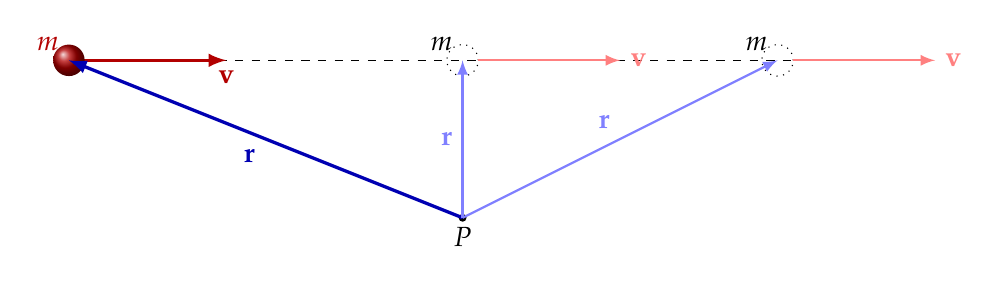
\begin{tikzpicture}
      \draw[dashed](-5,0)--(5,0);
      \draw[very thick,red!70!black,->](-5,0)--(-3,0) node[below]{$\mb{v}$};
      \tikzstyle{balloon}=[ball color=red!70!black];
      \shade[balloon] (-5,0) circle(.2) node[above left,red!70!black]{$m$};
      \fill[black] (0,-2) circle(.05) node[below]{$P$};
      \draw[very thick,blue!70!black,->](0,-2)--(-5,0)
      node[midway,below left]{$\mb{r}$};
      \uncover<2->{
        \draw[dotted](0,0) circle(.2) node[above left]{$m$};
        \draw[thick,red!50,->](.2,0)--(2,0)node[right]{$\mb{v}$};
        \draw[thick,blue!50,->](0,-2)--(0,0) node[midway,left]{$\mb{r}$};
      }
      \uncover<3->{
        \draw[dotted](4,0) circle(.2) node[above left]{$m$};
        \draw[thick,red!50,->](4.2,0)--(6,0)node[right]{$\mb{v}$};
        \draw[thick,blue!50,->](0,-2)--(4,0)node[midway,above left]{$\mb{r}$};
      }
    \end{tikzpicture}
  \end{center}
  \uncover<4>{
    Since there is no force and no torque acting on the object, both the linear
    momentum ($\mb{p}=m\mb{v}$) and angular momentum
    ($\mb{L}=\mb{r}\times\mb{v}$) are constant.
  }
\end{frame}



%TL1\begin{frame}{Example Problem}
%TL1  \textbf{Example 9:} A skater extends her arms (both arms!), holding a
%TL1  \SI{2.}{\kilo\gram} mass in each hand. She is rotating about a vertical axis
%TL1  at a given rate. She brings her arms inward toward her body in such a way that
%TL1  the distance of each mass from the axis changes from \SI{1.}{\metre} to
%TL1  \SI{.50}{\metre}. Her rate of rotation (neglecting her own mass) will?
%TL1\end{frame}
%TL1
%TL1
%TL1
%TL1\begin{frame}{Last Example}
%TL1  \textbf{Example 10:} A \SI{1.}{\kilo\gram} mass swings in a vertical circle
%TL1  after having been released from a horizontal position with zero initial
%TL1  velocity. The mass is attached to a massless rigid rod of length
%TL1  \SI{1.5}{\metre}. What is the angular momentum of the mass, when it is in its
%TL1  lowest position?
%TL1\end{frame}
%TL1
%TL1
%TL1\begin{frame}{Solving Rotational Problems}
%TL1  When solving for rotational problems like the ones described in the previous
%TL1  sections:
%TL1%  it is imperative to carefully draw a free-body diagram to account
%TL1%  for
%TL1%all the forces and torques acting on an object, as we have done in the previous
%TL1%examples. A few things to keep in mind:
%TL1  \begin{itemize}
%TL1  \item Draw a free-body diagram to account for all forces
%TL1  \item The direction of friction force is not always obvious
%TL1  \item The magnitude of any static friction force cannot be assumed to be at
%TL1    maximum.
%TL1  \item If the object is to change its rotational state, there must be a net
%TL1    torque causing it.
%TL1  \end{itemize}
%TL1\end{frame}
%TL1
%TL1
%TL1
%TL1\begin{frame}{Solving Rotational Problems}
%TL1  Once the free-body diagram is complete
%TL1  \begin{itemize}
%TL1  \item Breaks down the \emph{forces} into $\iii$, $\jjj$ and $\kkk$ components
%TL1  \item We have now three equations for translation, but it is likely that only
%TL1    \emph{one} direction will have forces:
%TL1
%TL1    \eq{-.3in}{
%TL1      \sum F_x=ma_x\quad\quad \sum F_y=ma_y\quad\quad \sum F_z=ma_z
%TL1    }
%TL1  \item And three equations for rotation, and torque is only applied in one
%TL1    direction (likely $\kkk$):
%TL1    
%TL1    \eq{-.3in}{
%TL1      \sum\tau_x=I_x\alpha_x\quad\quad \sum\tau_y=I_y\alpha_y\quad\quad 
%TL1      \sum\tau_z=I_z\alpha_z
%TL1    }
%TL1  \end{itemize}
%TL1\end{frame}
%TL1
%TL1
%TL1
%TL1\begin{frame}{Solving Rotational Problems}
%TL1  For rotational motion dynamics equation:
%TL1  \begin{enumerate}
%TL1  \item Relate the force(s) that causes rotational motion to the net torque
%TL1
%TL1    \eq{-.2in}{
%TL1      \tau=Fr
%TL1    }
%TL1  \item Substitute the expression for momentum of inertia (which has both mass
%TL1    and radius terms in it) into the equation for rotational motion
%TL1  \item Relate angular acceleration to linear acceleration, if applicable:
%TL1
%TL1    \eq{-.25in}{
%TL1      \alpha=\frac{a}R
%TL1    }
%TL1  \end{enumerate}
%TL1  Now there are two equations with force and acceleration terms. See handout
%TL1\end{frame}
%TL1
%TL1
%TL1  
%TL1\section{Rotational Kinetic Energy}
%TL1
%TL1\begin{frame}{Rotational Kinetic Energy}
%TL1  To find the kinetic energy of a rotating system of particles (discrete number
%TL1  of particles, or continuous mass distribution), we sum (or integrate) the
%TL1  kinetic energy of the individual particles:
%TL1    
%TL1  \vspace{-.3in}{\Large
%TL1    \begin{align*}
%TL1      K&=\sum_i\frac12m_iv_i^2=\frac12\left(\sum_i m_ir_i^2\right)\omega^2\\
%TL1      K&=\int\frac12v^2dm=\frac12\left(\int r^2dm\right)\omega^2
%TL1    \end{align*}
%TL1  }
%TL1  
%TL1  It's no surprise that in both case, rotational kinetic energy is given by:
%TL1  
%TL1  \eq{-.25in}{
%TL1    \boxed{K=\frac12I\omega^2}
%TL1  }
%TL1\end{frame}
%TL1
%TL1
%TL1
%TL1\begin{frame}{Kinetic Energy of a Rotating System}
%TL1  The total kinetic energy of a rotating system is the sum of its translational
%TL1  and rotational kinetic energies at its center of mass:
%TL1
%TL1  \eq{-.2in}{
%TL1    \boxed{K=\frac12mv_\text{CM}^2+\frac12I_\text{CM}\omega^2}
%TL1  }
%TL1  
%TL1  In this case, $I_\text{CM}$ is calculated at the center of
%TL1  mass. For simple problems, we only need to compute rotational kinetic energy
%TL1  at the pivot:
%TL1
%TL1  \eq{-.2in}{
%TL1    \boxed{K=\frac12I_\text{P}\omega^2}
%TL1  }
%TL1  
%TL1  In this case, the $I_\text{P}$ is calculated at the pivot.
%TL1  \textbf{IMPORTANT:} $I_\text{CM}\neq I_\text{P}$
%TL1\end{frame}
%TL1
%TL1
%TL1
%TL1\begin{frame}{Parallel Axis Theorem}
%TL1  \begin{columns}
%TL1    \column{.35\textwidth}
%TL1    \pic{1}{Steiner.png}
%TL1    
%TL1    \column{.65\textwidth}
%TL1    The \textbf{parallel axis theorem} relates the moment of inertia of an
%TL1    object along two different but parallel axis by:
%TL1
%TL1    \eq{-.2in}{
%TL1      \boxed{I=I_{\textrm{CM}}+md^2}
%TL1    }
%TL1  \end{columns}
%TL1\end{frame}
\end{document}
